\chapter{A guided tour of \alfa{}}
\label{chapstart}

{\sc Version of \today}

This chapter briefly presents the main features of the \alfa{} 
language and the basic operations of the \mmalfa{} environment.
Section~\ref{chapstart:examples} presents several examples of 
\alfa{} programs. In section~\ref{chapstart:basic}, we introduce
and illustrate a few basic manipulations of \alfa{} programs, 
whereas section~\ref{chapstart:advanced} presents more advanced
transformations. Structured programs are shown in~\ref{chapstart:sectstruct}.


\section{Examples of {\Alpha} programs}
\label{chapstart:examples}
For a complete description of the {\Alpha} language, refer to
appendix~\ref{alpha1} and~\ref{alpha2} or
to~\cite{wilde-tech94,Mauras89,DupontQuRi95}. We introduce the basic
features of the langage on the exemple of the matrix-vector
multiplication.

An {\Alpha} program is a {\em system}. \alfa{} variables are generalized
arrays which can have any shape (not just rectangles).  The set of
indices of the array is called the {\em domain} of the variable.
Example~\ref{ex1} below shows the declaration of a variable {\tt a}
whose domain is  the set of points $(i,j)$ in the triangle:  $0 \leq i \leq j$;
$j \leq 10$.

\begin{ex}
~\\
\texttt{a : \{i,j~|~ 0<= i <= j; j <=10 \} }
\label{ex1}
\end{ex} 

An \alfa{} system has input and output variables, it may have local
variables and also size parameters which allows parameterized programs
to be defined.  Variables are defined by a single equation (which
usually has the form of a recurrence equation). The {\tt case}
construct allows one to define different values in different parts of
the domain.

\begin{ex}
\texttt{
\\
a[i,j] = \\
case\\
\ \ \ \ \{| j = 0 \} : 0[];\\
\ \ \ \   \{| j > 0 \} : a[i,j-1]+1[];\\
         esac;
}
\label{ex2} 
\end{ex}

The {\Alpha} expression of example~\ref{ex2} defines the values of
{\tt a[i,0]} to be zero\footnote{Syntactic note: constants are zero
dimensionnal arrays hence the empty brackets in \texttt{0[]}. This
notation is the source of many syntax errors, and we plan to modify
it...} and recursively defines {\tt a} at all the other points in its
domain. This equation defines a variable {\tt a} such that {\tt
a[i,j]=j}. The above equation is printed in {\em array notation}.  The
real syntax of {\Alpha} is sligthly less readable but more consistent
and logical from a semantic point of view.  To illustrate this,
example~\ref{ex3} shows the same definition of {\tt a} in standard
notation.

\begin{ex}
{\tt 
~\\
a = \\
case\\
\ \ \ \ \       \{i,j | j = 0 \} : 0.(i,j->);\\
\ \ \ \ \      \{i,j | j > 0 \} : a.(i,j->i,j-1)+1.(i,j->);\\
    esac;\\
}
\label{ex3}
\end{ex}

Expression {\tt expr = a.(i,j->i,j-1)} should be read as {\em {\tt
a} composed with the dependency function} \texttt{f(i,j)=(i,j-1)}. In
other words, {\tt expr[i,j]} has value {\tt a[i,j-1]} at each point
\texttt{(i,j)} such that \texttt{(i,j-1)} is in the domain of {\tt a}. 
Similarly {\tt expr2 = 0.(i,j->)} means that {\tt expr2[i,j]} has
value \texttt{0} for all \texttt{(i,j)}.

Note also that there is no sequential in the different
computations: interchanging the two branches of the case in
example~\ref{ex2} would define exactly the same value for {\tt a}:
\alfa{} is therefore a declarative language.
The
evaluation order is implicit and there are tools for finding schedules
for a given program. As {\Alpha} is a functional language, the only
constraint that an evaluation order must follow is the data
dependencies between variables. In example~\ref{ex2},
obviously {\tt a[i,j]} must be computed after {\tt a[i,j-1]}.

More details on the langage can be found in
appendix~\ref{alpha1}. Figure~\ref{fig1} shows an \alfa{} program to
compute the multiplication of a matrix of size $n\times n$ and a vector
of size $n$.
\begin{figure}[htbp]
\begin{verbatim}
system prodVect: {N | N>1}
               (a : {i,j|1 <= i,j <= N} of integer; 
                b : {i|1 <= i <= N} of integer)
       returns (c : {i|1 <= i <= N} of  integer);
  var 
	C :  {i,j|1 <= i <= N; 0<= j <=N} of  integer;
  let
    C[i,j] = case
              {|j=0} : 0[];
              {|j>=1} : C[i,j-1] + a[i,j] * b[j];
             esac;
    c[i]=C[i,N];
  tel;   
\end{verbatim}
\caption{{\Alpha} program describing the matrix vector multiplication}
\label{fig1}
\end{figure}

\section{Basic manipulation of {\Alpha} programs}
\label{chapstart:basic}

This section presents the first commands that you should learn in
order to deal with {\Alpha} programs. Before reading this section, you
should have set the different environment variables necessary to use
the {\mmalfa{}} environment. This procedure is described in
appendix~\ref{install}.

There are several ways of using \mmalfa{}:
\begin{enumerate}
\item Using the notebook interface. Type \texttt{mathematica} under
\texttt{Unix}, or start \mma{}~3.0 in the Programs menu of 
Windows NT.
\item Using the \mma{} kernel directly. Type \texttt{math} under
\texttt{Unix}, or start \mma{}~3.0~Kernel in the Programs menu of 
Windows NT.
\item Using the \mma{} kernel via \texttt{emacs} (\texttt{Unix}
only).
\end{enumerate}

The second method is not recommended. The first one is easy, but
some people prefer using the third one. In the following, we shall
assume that we interact with the kernel (using the second
or the third method), but all commands we describe can also be
used in a notebook. 

Once {\mmalfa{}} is installed, start \mma{} and write an {\Alpha}
program (such as the one of figure~\ref{fig1} for instance) using your
favorite text editor. Say you called this file {\tt
prodVect.alpha}. The commands described in this section allow you to
{\bf load} your program into \mma{}, {\bf view} the program in
\mma{} (array notation or standard notation), {\bf save} the
program in another file, perform {\bf static analysis} and {\bf schedule}
the program. By the way, all these examples are alse available
in the \texttt{Getting-started} notebook accessible by the 
\texttt{Master} notebook of \mmalfa{}.


\subsection{Loading and viewing an {\Alpha} program}
When \mma{} is loaded, a few welcome messages about {\Alpha} are
printed out. 
Then one gets the usual \mma{} prompt:\\ {\tt In[1]:=
}\\ 
The name of the working directory can be printed out
by typing:\\
{\tt In[1]:=Directory[] }\\
If you see that this directory is not the one where you have put 
{\tt prodVect.alpha}, change it by typing:\\
{\tt In[2]:= SetDirectory[" the directory you want "] }\\

You can now {\bf load} the {\Alpha} program into \mma{}
by typing:\\
{\tt In[3]:= load["prodVect.alpha"]; }\\
Note that most often, \mmalfa{} commands should end with a semi-colon.
The reason is the following one: \mmalfa{} commands are \mma{} functions, 
which most often return a transformed \alfa{} program, expressed
as its AST. 
If you forget the {\tt ;} symbol,
\mma{} just prints out the result of the function evaluation, 
which sometimes may take a few pages... 
The side effect of \texttt{load} is to assign the AST  to 
the global \mma{} variable {\tt \$result}.

You can view the program that has been stored in {\tt \$result} by typing:\\
{\tt In[4]:= show[] } \\
By default, \texttt{show} pretty prints the program contained 
in {\tt \$result}, but more generally, \\\texttt{show[ var ]}\\would
pretty print the program contained in \mma{} variable \texttt{var}.

By the way, all \mma{} functions have an on-line documentation: 
\texttt{?show} gives the help on \texttt{show}. Commands
may have options. Type \texttt{Options[ command ]} to list
the options of \texttt{command} together with their default value.

You may have noticed that the program printed on the screen looks
different from the one of figure~\ref{fig1}: this program is in
standard notation. If you want to print it in array notation (which is
much more readable) you should evaluate: \\ {\tt In[6] := ashow[]}\\

To save the {\Alpha} program in another file, use
the command {\tt save} (or {\tt asave} which writes in array
notation).  For instance: \\ {\tt In[7]:= asave["myFile.alpha"] }\\
will write program of figure~\ref{fig1} in file {\tt
myFile.alpha}.
This command is needed if one wants to save
the content of \texttt{\$result} after some transformations. 

\subsection{Analyzing and simulating an {\Alpha} program}

Now that you have loaded an {\Alpha} program, you can start working on
it. Your first action should be to check it for so-called {\em static
errors} by using the command {\tt analyze}:\\ {\tt In[8]:=
analyze[]}\\ Information about possible errors of the {\Alpha} program
are printed out. If the analysis is successful, the result is {\tt
True}. The static analyzer of \alfa{} does essentially two verifications: 
it checks the type of expressions -- this is not a fantastic 
novelty, -- but it also checks that variables have a definition 
in any point of their domain definition. This second verification
is very powerful, and is much more original. 

Another interesting analysis tool is the {\tt scheduler}. It
finds (whenever possible) a linear schedule for your {\Alpha} program that
minimizes its execution time. The use of the scheduler is detailed in
subsection~\ref{schedule}. 

Suppose now that you want to evaluate the {\Alpha} program you just
loaded. There is no real compiler for {\Alpha} but we can generate
{\tt C} code that evaluates \alfa{} in a demand driven way. 
The command for generating {\tt C} code is {\tt writeC}:\\
{\tt In[9]:= writeC["prodVect.c","-p 10"] }\\ The {\tt "-p 10"}
argument indicates that the value of the parameter {\tt N} will be set
to 10 (the {\tt C} code is not parameter independent).
By
default, this program, once compiled, reads its input from the
standard input ({\tt stdin}) and prints on the standard output ({\tt
stdout}). 

\section{Advanced manipulation of {\Alpha} programs}
\label{chapstart:advanced}

In this section we briefly review a few more advanced manipulations of
{\Alpha}. Additional information is in the {\Alpha} tutorial and the
{\Alpha} reference manual (these documents are part of the \mmalfa{}
distribution).

\subsection{Pipelining}
Pipelining is a transformation widely used in systolic synthesis.
It is also called {\em localization} or {\em uniformization}.
It consists basically of replacing a broadcast 
by the pipeline of this value through all the computations that 
need it.  

For instance, in the program of figure~\ref{fig1}, we see (last 
term in the second branch of the {\tt case}) that 
{\tt b[j]} is used for the computation of {\tt C[i,j]} 
for all $i$, $0\leq i \leq N$. 

To introduce a new variable {\tt B1} which will pipeline the {\tt b[j]} 
value from the computation of {\tt C[j,0]} to 
{\tt C[j,1]}, ... , {\tt C[j,N]}, we
use the following command:\\
{\tt In[10]:= pipall["C","b.(i,j->j)","B1.(i,j->i+1,j)"]; }\\
In this expression, the first argument is the variable whose
equation is to be modified, the second argument is the
expression to be pipelined (standard notation is mandatory here)
and the last argument indicates the {\em direction} of the pipeline
as well as the name of the new variable introduced. 
After the
execution of this command, the program contained in {\tt \$result} is
the one shown in figure~\ref{fig2}.

\begin{figure}[ht]
\begin{verbatim}
system prodVect :{N | 2<=N}
                (a : {i,j | 1<=i<=N; 1<=j<=N} of boolean; 
                 b : {i | 1<=i<=N} of boolean)
       returns  (c : {i | 1<=i<=N} of boolean);
var
  B1 : {i,j | 1<=i<=N; 1<=j<=N; 2<=N} of boolean;
  C : {i,j | 1<=i<=N; 0<=j<=N} of boolean;
let
  B1[i,j] = 
      case
        {| i=1; 1<=j<=N; 2<=N} : b[j];
        {| 2<=i<=N; 1<=j<=N} : B1[i-1,j];
      esac;
  C[i,j] = 
      case
        {| j=0} : False[];
        {| 1<=j} : C[i,j-1] + a[i,j] * B1;
      esac;
  c[i] = C[i,N];
tel;
\end{verbatim}
\caption{{\Alpha} program of figure~\ref{fig1} after pipelining of {\tt b}
in the definition of \texttt{C}}
\label{fig2}
\end{figure}

Unlike previous transformations, pipelining changes the
{\Alpha} program, but the resulting program is equivalent to
the initial one. 
The modifications performed automatically by \texttt{pipeAll} are:
\begin{enumerate}
\item Determine the domain of {\tt B1} and add a
declaration for it.
\item Build the definition of {\tt B1} based on the dependency ({\tt (i,j->i+1,j)}) and the initialisation given ({\tt b.(i,j->j)}).
\item Replace the original expression ({\tt b.(i,j->j)}) by {\tt B1}.
\end{enumerate}

\subsection{Change of basis}
The change of basis is another important transformation in systolic
array design. It allows 
variables to be re-indexed, and is often used to map indices to time and space. 

In the example of figure~\ref{fig2}, suppose that we wish to express
the computations in a new index basis {\tt i',j'} such that {\tt i'=i+j}, 
{\tt j'=j}. We can perform the following change of basis:
\\ {\tt In[11]:= changeOfBasis["C.(i,j->i+j,j)"]; } \\ This simply
indicates that the transformation is to be applied to variable {\tt C}
and that the new coordinates in term of the old ones are given by
the linear function \texttt{(i,j->i+1,j)}.
Note that a change of basis is meaningful only if
this linear function admits an integral left inverse: in this
example, its left inverse is obviously \texttt{(i,j->i-1,j)}. The
resulting program is shown in figure~\ref{fig3}.

\begin{figure}[ht]
\begin{verbatim}
system prodVect :{N | 2<=N}
                (a : {i,j | 1<=i<=N; 1<=j<=N} of boolean; 
                 b : {i | 1<=i<=N} of boolean)
       returns  (c : {i | 1<=i<=N} of boolean);
var
  B1 : {i,j | 1<=i<=N; 1<=j<=N; 2<=N} of boolean;
  C : {i,j | j+1<=i<=j+N; 0<=j<=N} of boolean;
let
  B1[i,j] = 
      case
        {| i=1; 1<=j<=N; 2<=N} : b[j];
        {| 2<=i<=N; 1<=j<=N} : B1[i-1,j];
      esac;
  C[i,j] = 
      case
        {| j=0} : False[];
        {| 1<=j} : C[i-1,j-1] + a[i-j,j] * B1[i-j,j];
      esac;
  c[i] = C[i+N,N];
tel;
\end{verbatim}
\caption{{\Alpha} program of figure~\ref{fig2} after the change of basis on 
 {\tt C}}
\label{fig3}
\end{figure}

%\subsection{Substitution}
%{\tt To be written soon...}
\subsection{Normalization}
\label{normalization}
The normalization transformation simplifies an {\Alpha} program into a
{particular} normal form called {\em case-restriction-dependency}.
This function is very useful when one performs several automatic
transformations that may render the program less and less
readable. The command is simply: \\
{\tt In[12]:= normalize[];}\\This transformation is illustrated in the
\alfa{} tutorial.

\subsection{Scheduling}
\label{schedule}

The {\tt schedule} command looks for a schedule for an {\Alpha}
program.  The basic goal of the scheduler is to find a valid and good
evaluation order. Here, the term {\em good} depends on the
optimization criterion choosen: most often, it is the total evaluation
time of the program, but one may also consider other criteria.

The time is considered as a discrete single rate clock. The overall
idea of the scheduling process is to build a linear programming
problem (LP) and to solve it with a software tool: 
this may be \pip{}\cite{pip}, or \lpsolve{}\cite{lpsolve}, or even the \mma{}
linear solver. 

The \alfa{} scheduler provides several options to schedule 
a program. We consider here 
the simplest one (by default), called 
{\em  monodimensional affine-by-variable schedule}. 
This esoteric name means 
that the evaluation date $T_A(i,j)$ of a given computation
\texttt{A[i,j]}  
is given by an affine
function of the indices and parameters:\\
\centerline{ $T_{A}(i,j) =
\tau^i_{A} i + \tau^j_{A} j+ \tau^N_{A} N +
\alpha_{A}$} where $N$ is a 
parameter of the {\Alpha} program.
The coefficients of this function
are (in general) different for each variable in the system 

The command to schedule a program is :\\ 
\texttt{schedule[]}\\By default, it schedules {\tt \$result}
and the resulting schedule is
placed in a global variable named {\tt \$schedule}. 

The \texttt{schedule} function has many options 
(type {\tt Options[schedule]} for further information.)
Some uses of the function {\tt schedule} are:
\begin{itemize}
\item {\tt schedule[]}\\ find an affine by variable schedule  for {\tt
\$result} which minimizes the global execution time and assign it to
{\tt \$schedule}.
\item {\tt schedule[sys]}\\ find an affine by variable schedule for
the {\Alpha} system {\tt sys} which minimizes the global execution
time and assign it to {\tt \$schedule}.
\item {\tt
schedule[\{option1->value1,\ldots,optionn->valuen\}]}\\
find a schedule for {\tt \$result} which respects the chosen options and
assign it to {\tt \$schedule}.
\item {\tt
schedule[sys,\{option1->value1,\ldots,optionn->valuen\}]}\\
find a schedule for the {\Alpha} system {\tt sys} which respects the chosen options and
assign it to {\tt \$schedule}.
\end{itemize}
The schedule function is explained in more detail in
the scheduler documentation
given in file:
\begin{verbatim}
$MMALPHA/doc/user/docSched.dvi
\end{verbatim}

\section{Structured  {\Alpha} programs}
% Macros pour la syntaxe
\label{chapstart:sectstruct}

\index{genericity}\index{structured programming}\index{program structures}\index{structures of programs}
\alfa{} programs can be structured: this section explains 
how this can be done. 

\subsection{Simple structures} 
Let us write an {\alfa} program for the addition of two integers
(or fixed-point numbers) expressed as bit vectors.  A binary
adder is classically described as a sequence of \emph{full adder}
operations with the propagation of a carry bit from one full adder to
the next one, as shown in Fig.\ref{binaryadder}.
\index{adder}\index{binary addition}

\begin{figure}[!ht]
  \centerline{
    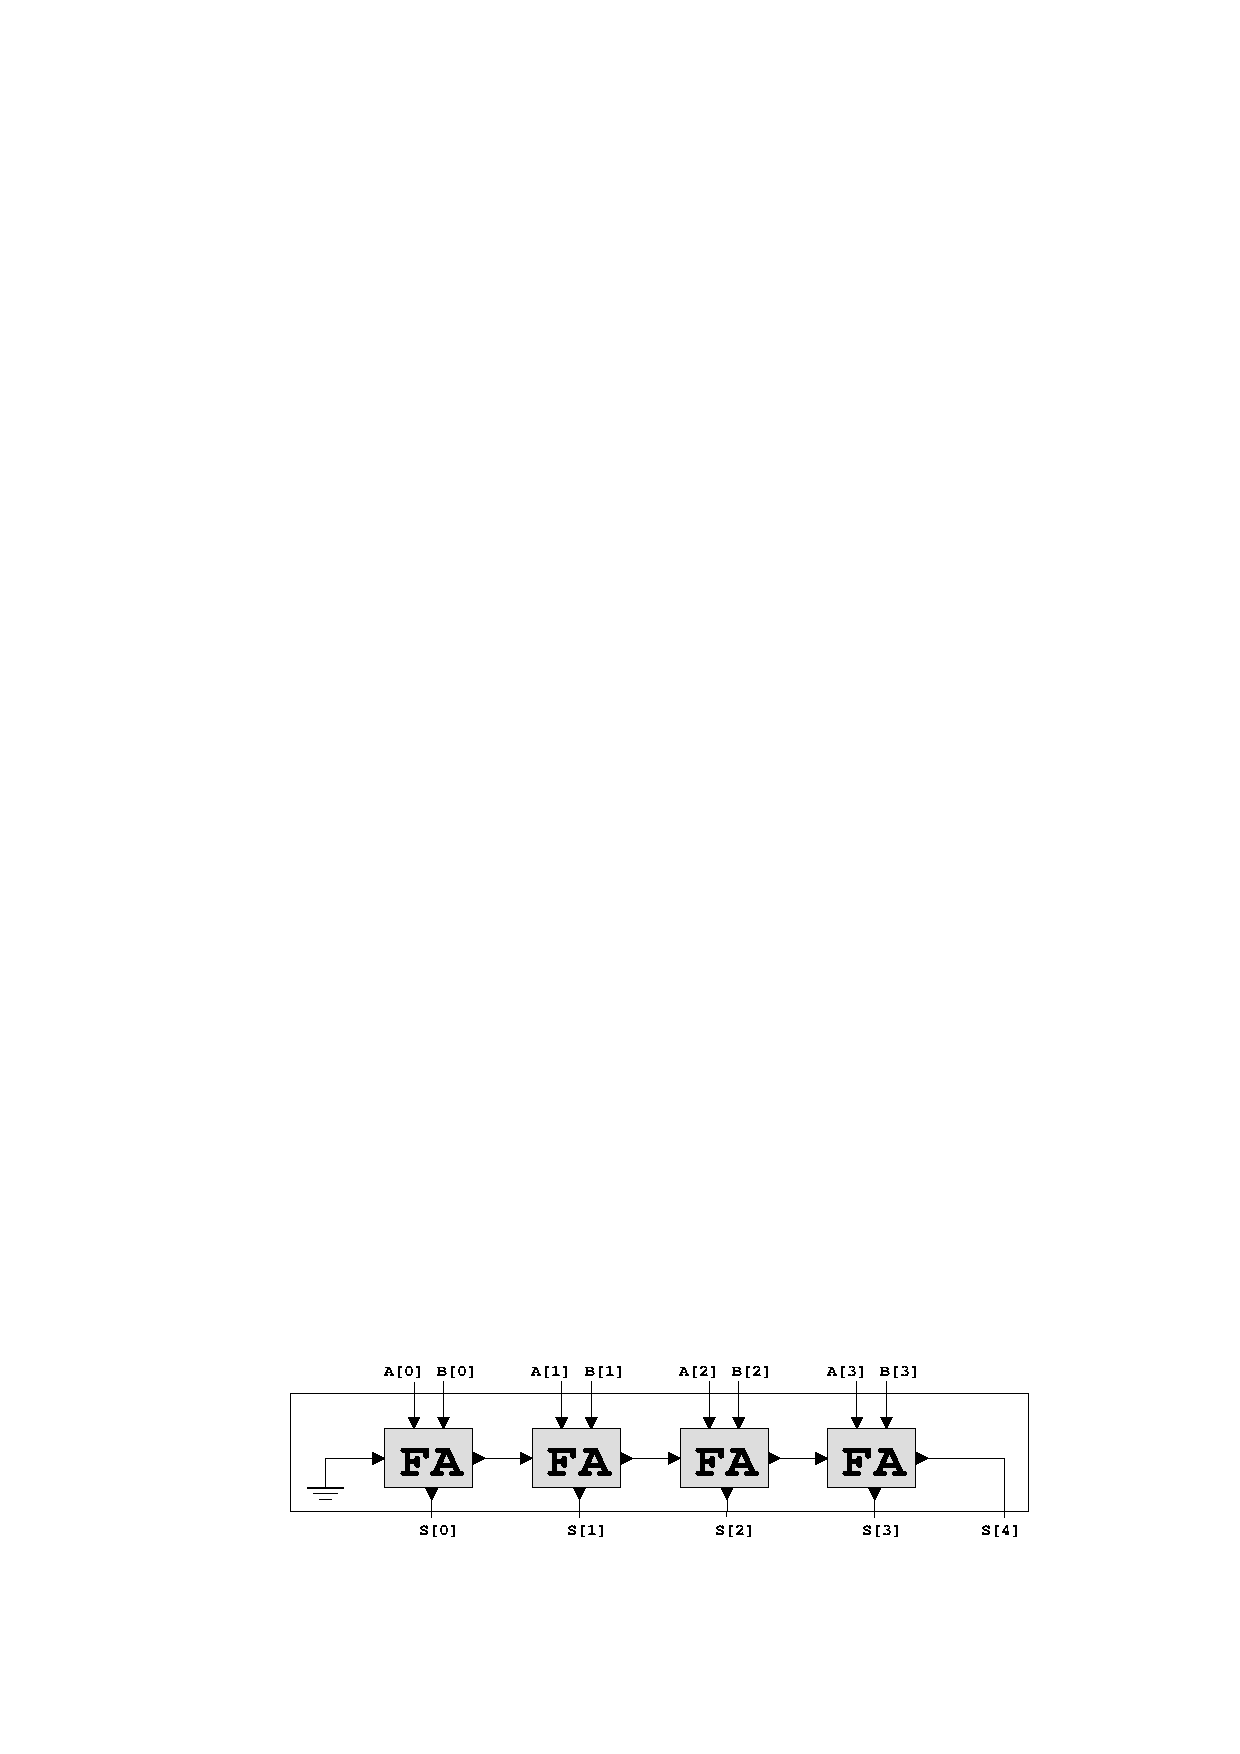
\includegraphics{adder.pdf}
  }
\caption{Addition of two integers (coded as bit vectors), using \emph{full adders}\label{binaryadder}}
\end{figure}

The following \alfa{} system describes a \emph{full adder}:
\index{full adder}
\begin{verbatim}
      system FullAdder (A,B,Cin : boolean) 
               returns (X,Cout : boolean);
      let
        X = A xor B xor Cin;
        Cout = (A and B) or (A and Cin) or (B and Cin);
      tel;
\end{verbatim}

To build an adder using this program, we need to 
instanciate a collection of such system,
as shown in Fig.\ref{binaryadder}. The shape of this collection may
be expressed as the {\alfa} domain \texttt{\{b|0<=b<W\}} where
\texttt{W} is a size parameter giving the number of bits of the
adder.
\index{use statement}

The \textbf{use} construct of {\alfa} allows precisely that: the
following system describes in {\alfa} the adder given in
figure~\ref{binaryadder}:
\index{adder}\index{binary addition}

\begin{verbatim}
system Plus: {W|W>1} (A,B: {b| 0<=b<W} of boolean)              -- 1       
             returns (S : {b| 0<=b<=W} of boolean);             -- 2       
var                                                             -- 3       
  Cin, Cout, X : {b| 0<=b<W} of boolean;                        -- 4       
let                                                             -- 5       
  Cin[b] =                                                      -- 6       
    case                                                        -- 7       
      {| b=0} : 0[];                                            -- 8       
      {| b>0} : Cout[b-1];                                      -- 9       
    esac;                                                       -- 10      
  use {b| 0<=b<W} FullAdder[] (A,B,Cin) returns(X, Cout);       -- 11      
  S[b] =                                                        -- 12      
    case                                                        -- 13      
      {| b<W} : X;                                              -- 14      
      {| b=W} : Cout[W-1];                                      -- 15      
    esac;                                                       -- 16      
tel;                                                            -- 17      
\end{verbatim}

\index{use statement}
In this system, line 11 reads as follows: 
\begin{quote}
``Use (or instantiate)
a collection of
instances of the subsystem \texttt{FullAdder}. This collection has the
shape of the extension domain\index{extension domain} \verb!{b| 0<=b<W}! and is thus indexed
by index \texttt{b}. Let the inputs of the \texttt{b}-th instance be
the variables \texttt{A}, \texttt{B} and \texttt{Cin} at point
\texttt{b}, and similarly let the outputs of this collection of
instances be the variables \texttt{X} and \texttt{Cout}.''
\end{quote}
Lines~6-10 describe the carry propagation, and lines~12-16
define the output of this binary adder.

\index{dimension extension}
In other words, line~11 is a shortcut for the following equations,
which are those of the system \texttt{FullAdder} whith the dimension
of the variables extended from zero to one:

\begin{verbatim}
        X[b] = A[b] xor B[b] xor Cin[b];
        Cout[b] = (A[b] and B[b]) or (A[b] and Cin[b]) or (B[b] and Cin[b]);
\end{verbatim}


\subsection{Syntax of the \emph{use} construct}

\index{use syntax}
The \textbf{use}\ construct appears at the syntactic level of an
equation, since it is basically a shortcut for a set of
equations. Here is the general syntax of an equation/use (see
appendix~\ref{alpha1} for the meta syntax):
{\tt
\begin{tabbing}
xxx\= xxx\= xxx\= xxx\= xxx\= xxx\= xxx\= xxx\= xxx\=  \kill
\textsl{Equation} ::=\\
\>\> \textsl{Identifier} = \textsl{Expression} ;\\
\> \Alt\ \> use \Opt{ \textsl{ExtensionDomain}} \textsl{Identifier}\\
\>\>\>\>\>\> \Opt{[\textsl{ParamAssignment} ]} \\
\>\>\>\>\>\>( \textsl{ExpressionList} )\\
\>\>\> returns\>\>\> ( \textsl{IdentifierList} ) ;
\end{tabbing}
}
 
\index{parameter assignation}\index{assignation of the
parameters}\index{parameters}
In this syntax we see that there is an optional \emph{parameter
assignment} which is discussed in the following.
In the previous addition the subsystem \texttt{FullAdder} has
no parameters, and the parameter assignment is therefore empty. 

\subsection{Manipulating structured programs}

A structured program is stored in {\mmalfa{}} as a {\mma{}} list of
systems called a \emph{library}. The default library is stored in the
global variable \verb!$library!.\index{$library}

A structured program may be written in one single file or several
distinct files.  In the former case the \texttt{load[]} function
returns a library composed of all the systems contained in the file,
and stores this library in \verb!$library!. %$ 

If the program is stored in several files, it is the responsability of
the user to build a proper library, i.e. a {\mmalfa{}} list of all the
systems needed by the hierarchical structure of the program. For this
purpose, the user will typically use {\mmalfa{}} list manipulating
functions such as \texttt{Join[], Append[]}, etc.\index{structured
programs}

In addition, two functions, \texttt{putSystem[]} and
\texttt{getSystem[]}, may be used to extract a system from a library
and to put back a modified system in a library. Typically a
system is extracted from the library as the {\em current}
system, modified by some program
transformation, and then put back in the library.\index{putSystem[]}\index{\getSystem[]}

\subsection{Program transformations associated with structures}

Most \mmalfa{} functions handle parameterized programs and \emph{use}
statements. There are, however, some major exceptions such as the
\texttt{writeC[]} translator \index{writeC[]} which generates code
only for flat {\Alpha} programs without subsystems. 
\mmalfa{}
provides functions to transform a structured program
into a ``flat'' equivalent one~:

\begin{itemize}
\item \texttt{assignParameterValue[]} \index{assignParameterValue[]}
gives a value to a size parameter, i.e. it refines a generic system
into a specialized one.
\item \texttt{inlineSubSystem[]} \index{inlineSubSystem[]} expands a
\emph{use} statement, replacing it with the equations of the
corresponding subsystem, properly modified to take the dimension
extension into account.\index{flattening a structured program}
\item \texttt{inlineAll[]} \index{inlineAll[]} recursively flattens a
structured {\alfa} program.
\end{itemize}
For more information see 
the subsystem documentation
\begin{verbatim}
$MMALPHA/doc/user/SubSystems.dvi
\end{verbatim}

\section*{Appendix: The polyhedral library}
\label{polylib}
See~\cite{Wilde93}(\texttt{http://www.irisa.fr/EXTERNE/bibli/pi/pi785.html}


